\documentclass[11pt]{report}
\title{Implementation of the Streamlet Consensus Algorithm in Blockchain}
\author{
Luís Viana    \\
\texttt{fc62516}  \and
Guilherme Santos      \\
\texttt{fc62533} 
\date{\today}
}
\usepackage[left=1in,right=1in,top=1in,bottom=1in]{geometry}
\usepackage{tikz,pgfplots}
\usepackage{subfig}
\usepackage{caption}
\usepackage{amsmath}


\begin{document}

\maketitle
\counterwithout{section}{chapter}
\section{Introduction}
The project consists in the implementation of the Streamlet consensus algorithm.  The programming language used for this project was C\#, supported with the use of Protocol buffers (Google's language-neutral, platform-neutral, extensible mechanism for serializing structured data).  

The configuration of the project followed a 5 node architecture, being easily upscaled by the addition of new lines of \texttt{ip:port} to the \texttt{ips.txt} file.  

For the selection of the epoch’s leader we instantiated a random with the same seed in all nodes and generated a new value every epoch for an arbitrary but certain decision shared by all nodes.

For the implementation of the data structures defined in the \texttt{proto\_file.proto} file, we used the following composition, as mainly suggested in the project description, with the exception of the simplification of the Transactions representation.

\begin{itemize}
    \item Block: Hash (bytes), Epoch (integer), Length (integer), Transactions (string).  
    \item Message: Type (Propose, Vote, Echo), Content (Message or Block), Sender (integer)
\end{itemize}

The connection between nodes is done via instantiation of a TCPClient for each node, including itself (for the implementation of the URB-Broadcast). The exchange of messages between nodes is done via NetworkStreams. 

Our implementation follows the requested basic protocol without fault tolerance or desynchronization of nodes. The code output is represented in the image below. 

\vspace{20pt}
\begin{figure}[h]
    \centering
    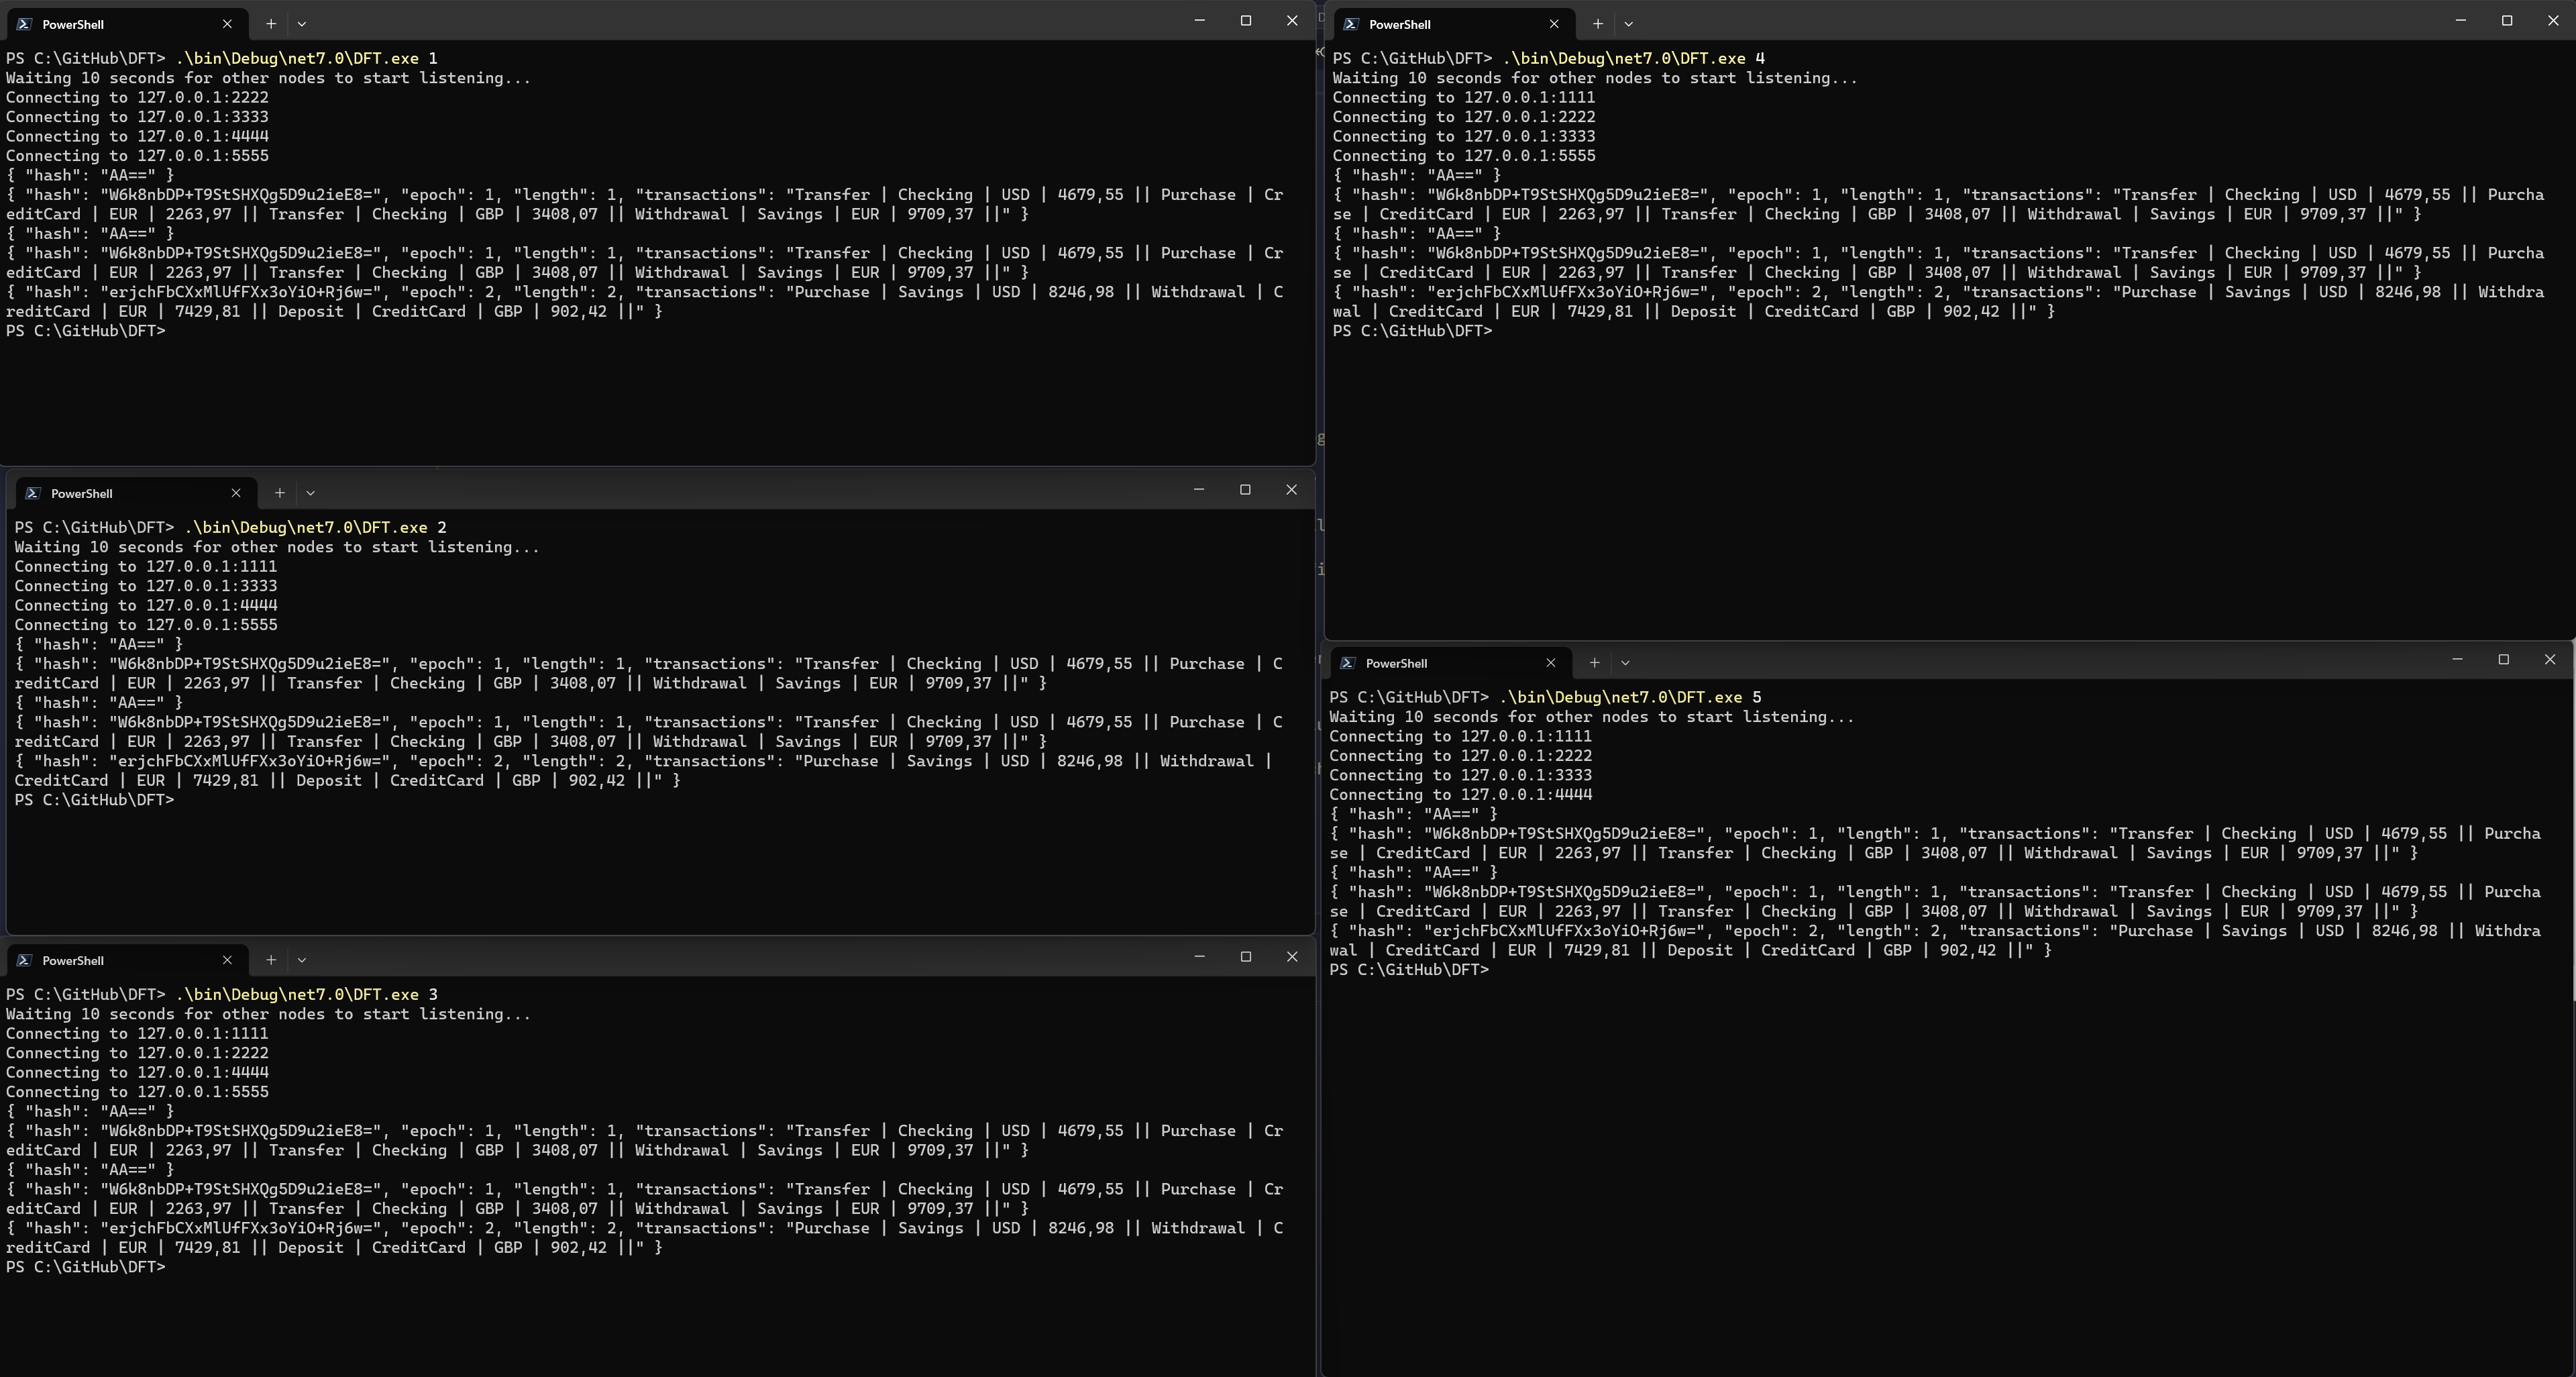
\includegraphics[width=1\textwidth]{5nodes.png}
    \caption{5 nodes running the Streamlet consensus algorithm.}
\end{figure}
\vspace{20pt}


\pagebreak
\section{Implementation}
\subsection{Uniform Reliable Broadcast Protocol:}
For the broadcast used in the propose and vote actions we implemented the Uniform Reliable Broadcast Protocol, where the node only sends the message to itself, and upon its reception, it sends to every other node excluding the sender of the message, via a call to the Echo function, the code of which is provided below. 

\vspace{20pt}
\begin{figure}[h]
    \centering
    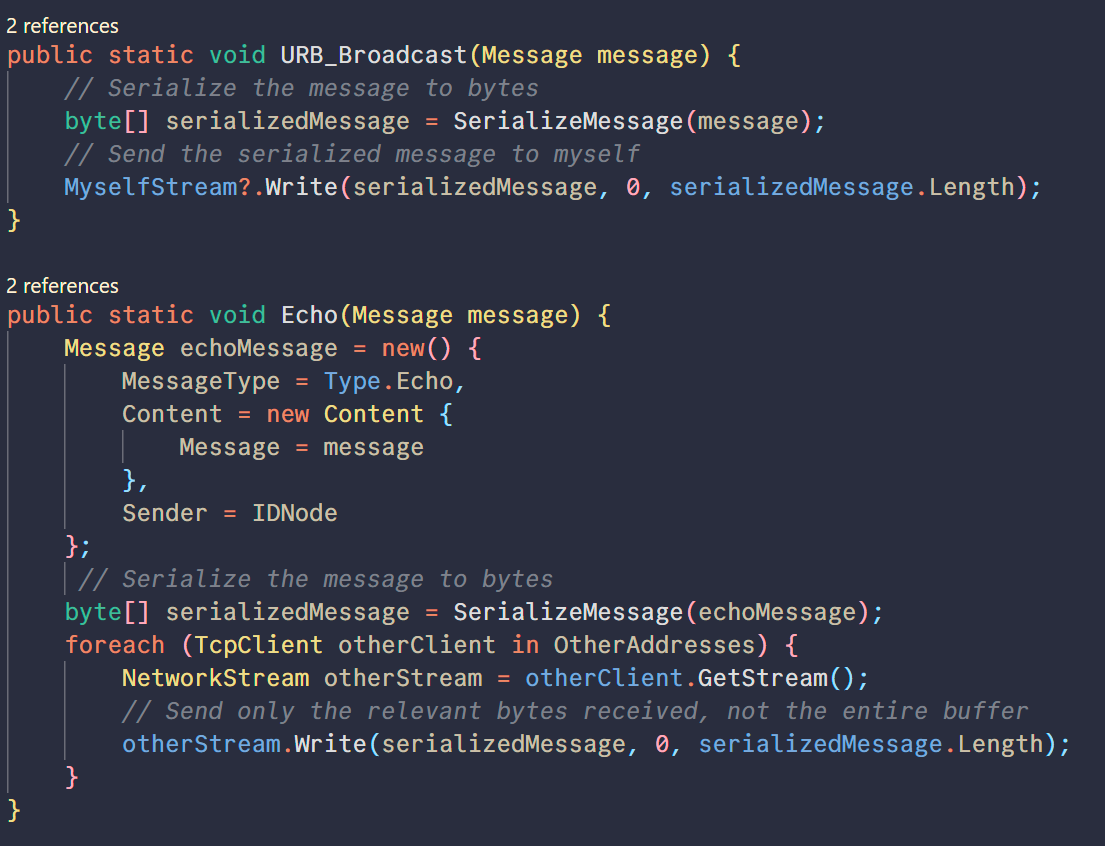
\includegraphics[width=0.6\textwidth]{broadecho.png}
    \caption{URB-Broadcast and Echo functions.}
\end{figure}
\vspace{20pt}

\vspace{20pt}
\begin{figure}[h]
    \centering
    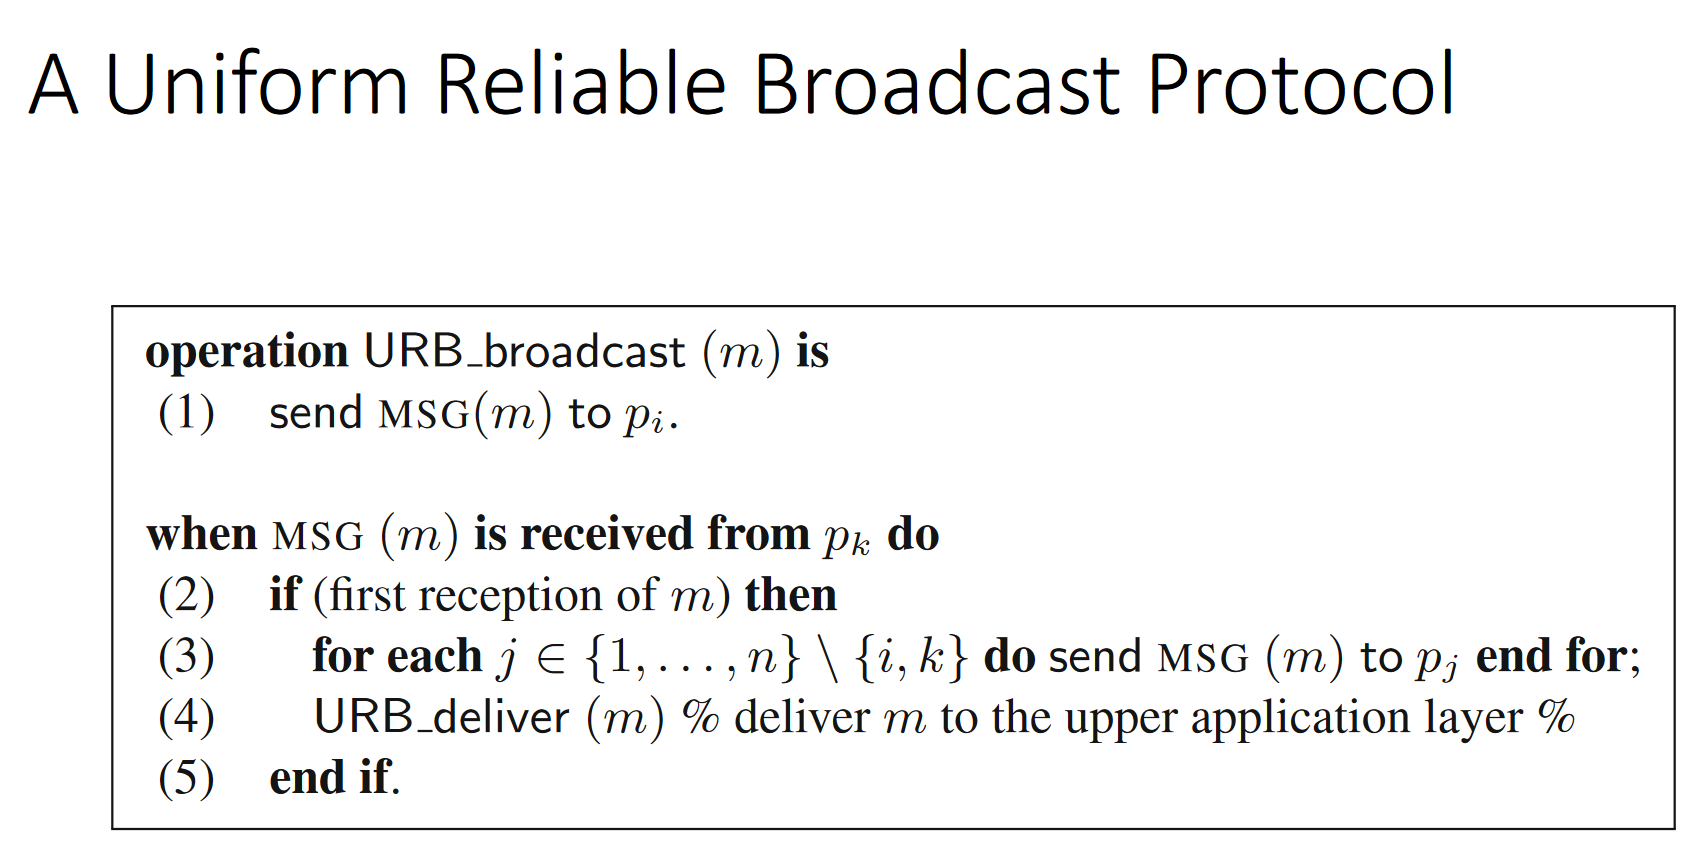
\includegraphics[width=0.6\textwidth]{urb.png}
    \caption{URB-Broadcast algorithm.}
\end{figure}
\vspace{20pt}

\pagebreak

\subsection{Saving of Echo Contents:} \label{2.2}

We save the contents of the echo to avoid receiving duplicate echo content across epochs.

\subsection{Clearing List at Start of Epoch:}

To improve performance, we use an approach of clearing the list of the received messages at the start of each period. This optimization assures that we start from scratch, avoiding redundant data processing from earlier epochs and optimizing memory use.


\subsection{Restricting Voting to Nodes Receiving Echo:}

To improve the voting process, only nodes that receive the echo of the proposed block are allowed to vote. This decision is especially important for avoiding the leader vote because it already has the real proposed block via URB broadcast, therefore it will not receive the echo of the proposed as stated in \ref{2.2}.

\subsection{Implementation of \texttt{CheckFinalizationCriteria()}:}

The method was developed to identify the most recently completed block and act as a reference point for subsequent blockchain additions. Blocks that do not satisfy or are shorter than the length of the last finished block are considered invalid.



\end{document}

